\documentclass[dvipdfmx, titlepage, t]{jsarticle}

% \usepackage{geometry}
\usepackage[dvipdfmx]{graphicx}
\usepackage{ascmac}
\usepackage{amsmath}
\usepackage{amssymb}
\usepackage{minted}
\usepackage{listings}
% \usepackage[utf8]{inputenc}
% \usepackage{listingsutf8}
\usepackage{newfloat} % newfloat パッケージを読み込む
\usepackage{caption}
\usepackage{float}
\usepackage{fix-cm}
\usepackage{svg}
\usepackage{enumitem}

\usepackage{hyperref}
% for hyperref
\usepackage{pxjahyper}
\hypersetup{
    dvipdfmx,
	colorlinks=false, % リンクに色をつけない設定
	bookmarks=true, % 以下ブックマークに関する設定
	bookmarksnumbered=true,
	pdfborder={0 0 0},
	bookmarkstype=toc
}

% \lstset{
%   basicstyle={\ttfamily},
%   identifierstyle={\small},
%   inputencoding=auto,
%   commentstyle={\small\sffamily},
%   keywordstyle={\small\bfseries},
%   ndkeywordstyle={\small},
%   stringstyle={\small\ttfamily},
%   frame={tb},
%   breaklines=true,
%   columns=[l]{fullflexible},
%   numbers=left,
%   % xrightmargin=0zw,
%   % xleftmargin=3zw,
%   numberstyle={\scriptsize},
%   firstnumber=auto,
%   stepnumber=1,
%   numbersep=5pt,
%   lineskip=1ex
% }

% 新しい浮動体「listing」を定義
\DeclareFloatingEnvironment[
    fileext=lol,       % List of Listings ファイルの拡張子 (List of Listings を作成する場合)
    name=Listing,      % キャプションの接頭辞 (例: "Listing 1")
    placement={!htbp}, % フロートの配置オプション (お好みで調整してください)
    within=section     % 番号付けをセクションごとにする場合 (例: Listing 1.1) (任意、不要なら削除)
]{program}

\setminted{
  mathescape,              % 数式モードへのエスケープを許可 (必要なら)
  % basicstyle やフォント関連
  fontsize=\small,         % 全体のフォントサイズ (listings の \small に合わせる試み)
                           % \ttfamily は minted のデフォルトに近いが、日本語対応の等幅フォントを
                           % LaTeX 側で \ normaalfont や \ttdefault に設定しておくのが理想
  % frame
  frame=lines,             % 上下に線を引く frame=tb に近いものとして lines (上下左右に線)
  framesep=2mm,            % 枠線とコードの間隔 (調整が必要)
  % breaklines
  breaklines=true,         % 自動折り返し
  % numbers
  linenos=true,            % 行番号を左に表示
  firstnumber=auto,        % 行番号を開始行に合わせる
  numbersep=5pt,           % 行番号とコードの間隔
  % stepnumber=1,          % linenos=true で通常1ステップ
  % highlight と Pygments スタイル
  % minted では Pygments のスタイルを使います。
  % style=friendly のようにスタイル名を指定できます。
  % デフォルトのスタイルでキーワードが太字になるか確認。
  % commentstyle や keywordstyle の LaTeX コマンド直接指定はできません。
  % Pygments のスタイルでこれらがどのように見えるか確認し、
  % 必要ならカスタムスタイルを作るか、別の既存スタイルを選びます。
}

\title{title}
\author{情報学群 \\ 1270328 佐藤謙成}
\date{\today}

\begin{document}
\maketitle

\begin{abstract}
    
\end{abstract}
\section{全体の目的}
\subsection{第六回の目的}
    第六回では,地球に到達する光を分析することにより,恒星の動きを知ることを目的とする.恒星がどの程度の速度で地球から遠ざかっているのかを算出し,観測されたスペクトルを描画する.また,単一の恒星についての分析と複数の恒星についてどのよう分析を行い,~~する.
\subsection{第七回の目的}
    第七回では,次回の眼球運動継続実験の準備としてMatLab及びPsychotoolboxを用いてプログラムを作成する.本課題では,被験者が左右に提示される顔画像の魅力を判断し,キー押しで反応する二者択一の選択課題を 2 試行行う実験環境を構築することである.
\subsection{第八回の目的}
\subsection{第九回の目的}
    第八回では,EyeLink II によって過去に測定された眼球運動実験のデータをプログラムを用いて解析することである.被験者が左右の顔画像のどちらかを選択する際に,選択した顔画像んいどの程度視線を向けていたかの確率を時間経過とともにグラフかすることを目的とする.
\subsection{第十回の目的}
\section{方法}
\subsection{第六回の方法}
    \inputminted[linenos, firstline=1, lastline=2, frame=lines, fontsize=\small]{matlab}{code/Exp3_6_Matlab.m}
    \ref{lst:exp3_6_load}では,まず starData というデータファイルを読み込み,\mintinline{matlab}|size(spectra,1)| で各スペクトルに含まれる観測点の数を取得する.

    次に,恒星 HD94028 のスペクトルを抽出する.それが以下のコード \ref{lst:exp3_6_s}である.
    \inputminted[linenos, firstline=14, lastline=19, frame=lines, fontsize=\small]{matlab}{code/Exp3_6_Matlab.m}
    ここでは,両軸対数スケールで出力するために関数 loglog を用いている.また,恒星 HD94028 のスペクトルはベクトル s に格納する.

    ベクトル s に格納された値を用いて水素アルファ線の波長を求める.コード \ref{lst:exp3_6_alpha} では, s の最小値が水素アルファ線であることを利用して \mintinline{matlab}|min(s)| で求めている.関数 min はここでは 2つの値を出力することができる.一つ目の値が水素アルファ線の値で二つ目の値がそのインデックスとなる.

    \inputminted[linenos, firstline=20, lastline=23, frame=lines, fontsize=\small]{matlab}{code/Exp3_6_Matlab.m}

    特定した水素アルファ線に対して点を追加するためのコードがコード\ref{lst:exp3_6_hold}である. ここでは, \mintinline{matlab}|hold on| を記述することで既存のグラフに点を追記することができ, \mintinline{matlab}|hold off| で追記を終了することができる.今回は,水素アルファ線の値の部分にマーカーサイズが 8 の赤い正方形をプロットする.
    \inputminted[linenos, firstline=24, lastline=27, frame=lines, fontsize=\small]{matlab}{code/Exp3_6_Matlab.m}
    
    赤方偏移係数と星が地球から遠ざかる速度を求める.赤方偏移係数は係数を $z$ としたときに $z = \dfrac{\lambda Ha }{656.28} - 1$ で求めることができるため,これを実装する.速度に関しては,赤方偏移係数に光速の値をかけることで求めることができる.
    \inputminted[linenos, firstline=29, lastline=31, frame=lines, fontsize=\small]{matlab}{code/Exp3_6_Matlab.m}

    % svgに変更しよう
    \begin{figure}[H]
        \centering
        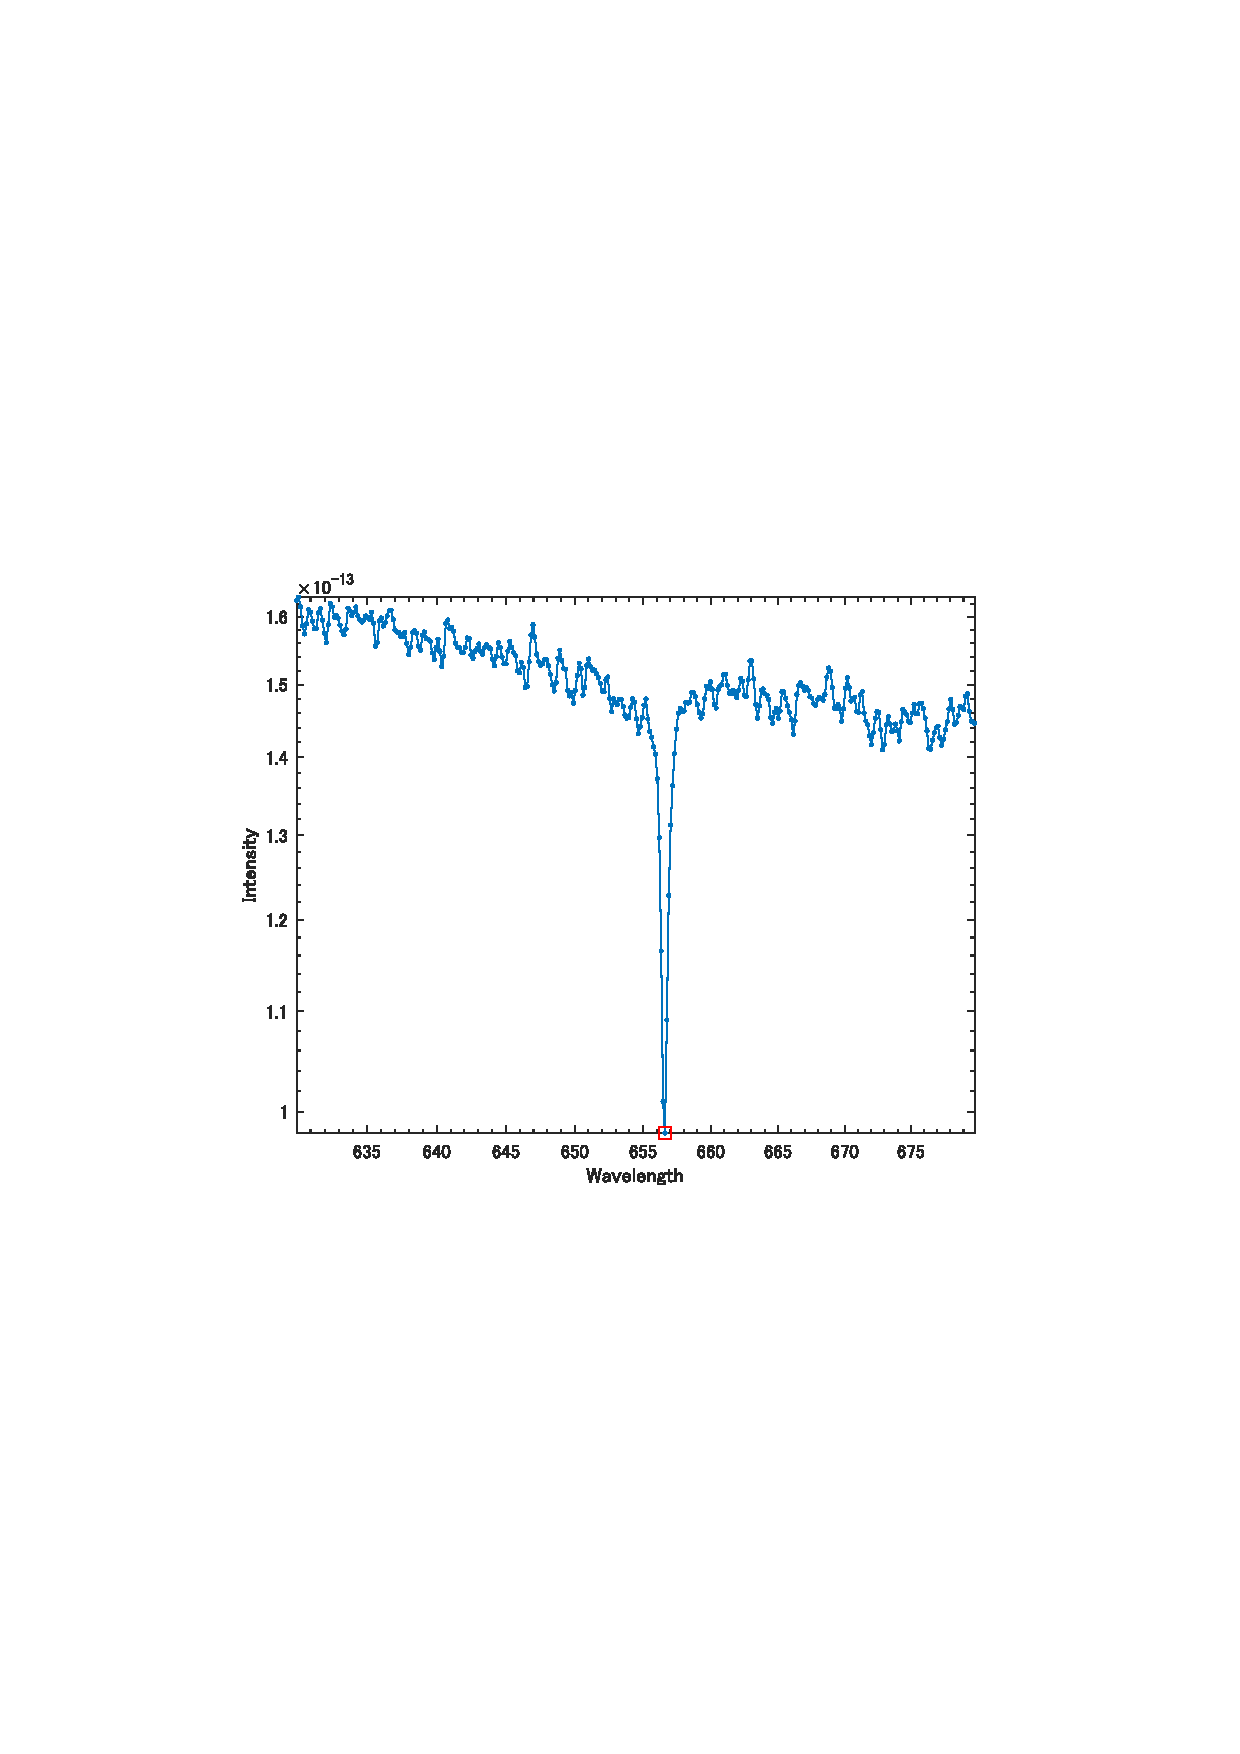
\includegraphics[width=0.5\textwidth]{figure/stellar1.pdf}
        \caption{恒星 HD94028 のスペクトルと水素アルファ線}
        \label{fig:exp3_6_spectra}
    \end{figure}

    ここから,各星の水素アルファ線を求める.行列の各行に対して最小値とそのインデックスを計算する.これは \mintinline{matlab}|min(spectra(:,:))| で求めることができる.また,各星の Ha の波長を \mintinline{matlab}|lambda(idx)|で求め,その値を用いて赤方偏移係数と速度を求める.

    \inputminted[linenos, firstline=11, lastline=15, frame=lines, fontsize=\small]{matlab}{code/Exp3_6_2_Matlab.m}

    この各星で求めた値を1つの図にまとめるプログラムで出力する.全ての星のスペクトルを一つのグラフに目止めて描画し,青方偏移か赤方偏移を視覚的に区別し,どの線がどの星に対応するかを明確にする.各星について速度が 0 以下の場合は青方偏移,0 より大きい場合は赤方偏移と判断するため,if文を用いて条件分岐を行う.また,その条件分岐を各星に対して行うために for 文を用いる.
    \inputminted[linenos, firstline=16, lastline=27, frame=lines, fontsize=\small]{matlab}{code/Exp3_6_2_Matlab.m}

    % svgに変更しよう
    \begin{figure}[H]
        \centering
        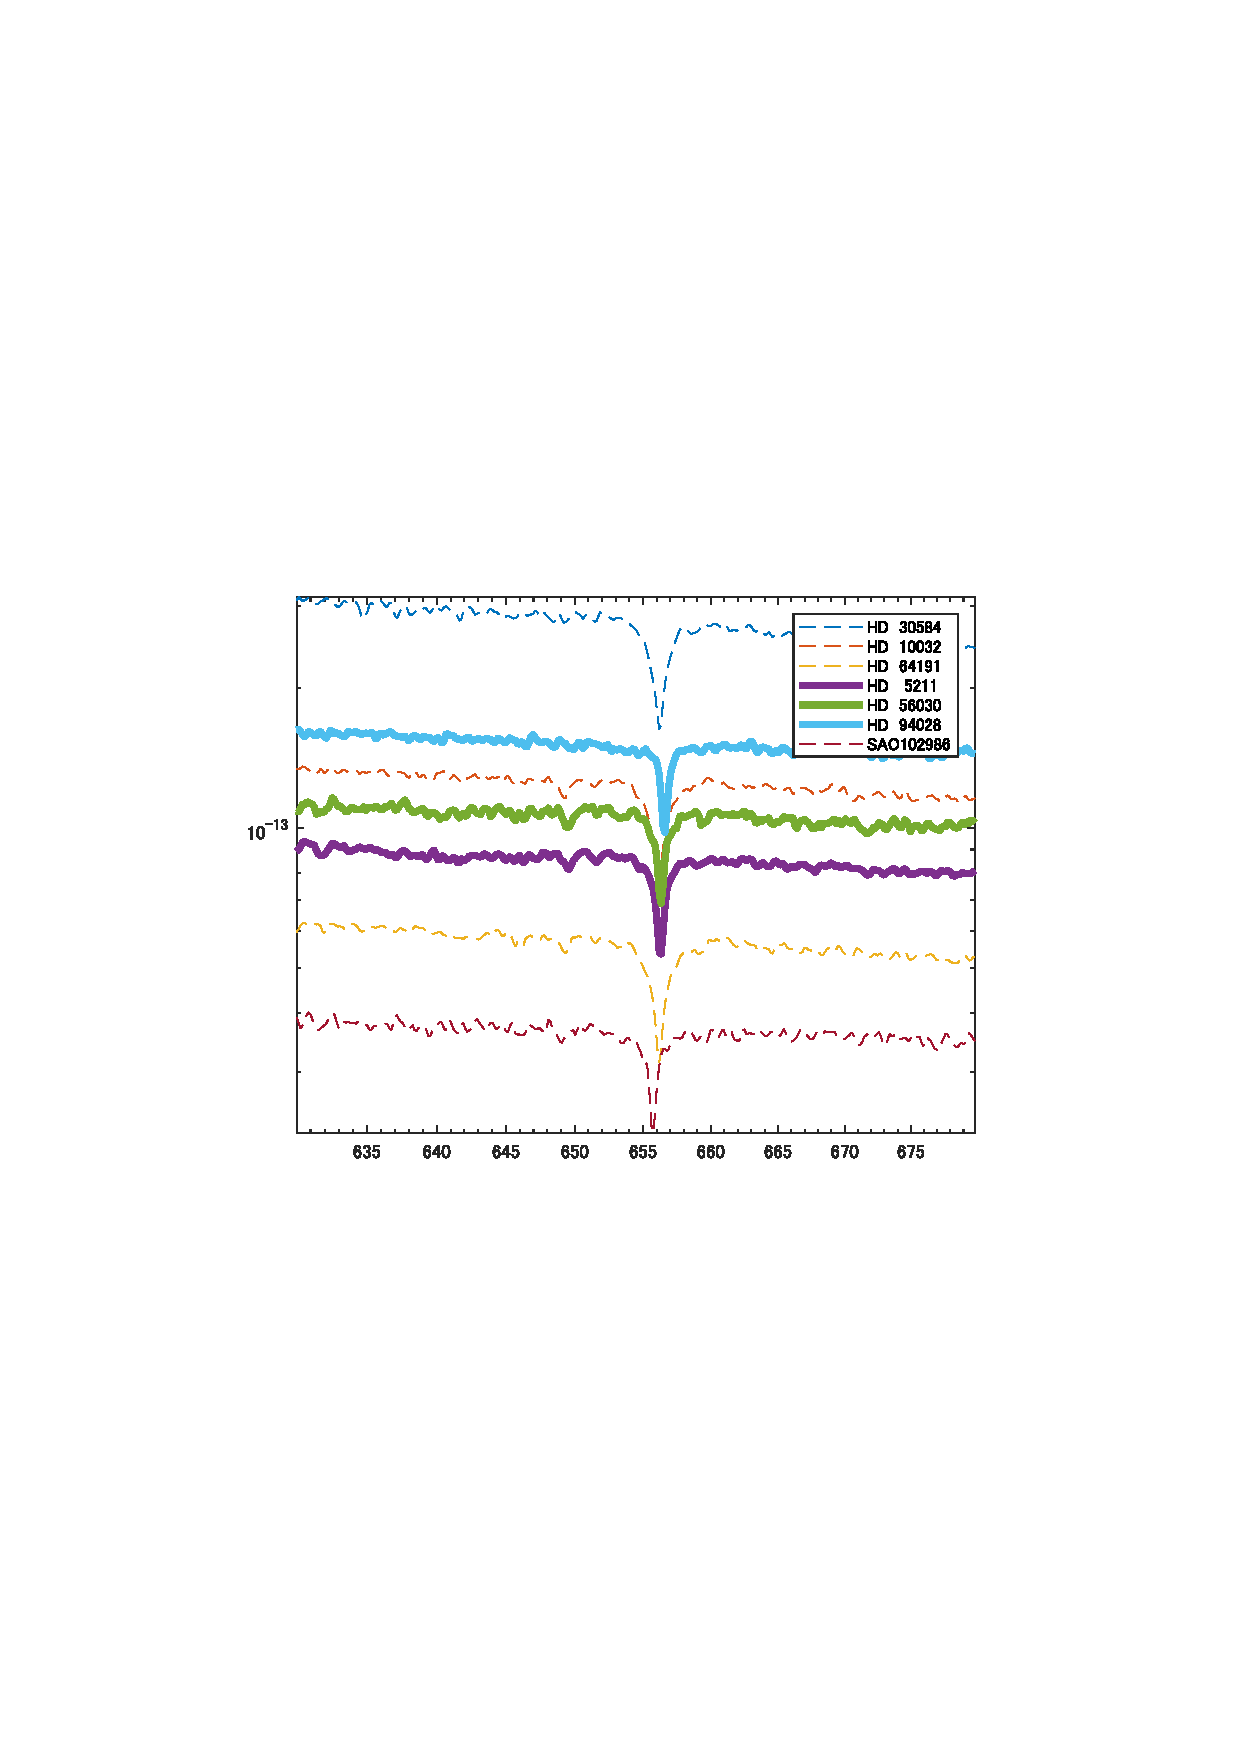
\includegraphics[width=0.5\textwidth]{figure/stellar2.pdf}
        \caption{各星のスペクトルと水素アルファ線}
        \label{fig:exp3_6_spectra2}
    \end{figure}

\subsection{第七回の方法}
    まず,刺激呈示環境を構築する.まず,背景色を白色とするために \mintinline{matlab}|bgcolor = 255| と設定する.刺激画像の大きさは 640 $\times$ 480 とするので 高さは \mintinline{matlab}|h = 640| とし,幅は \mintinline{matlab}|w = 480| とする.

    \begin{program}
    \inputminted[linenos, firstline=5, lastline=12, frame=lines, fontsize=\small]{matlab}{code/Exp3_7_Matlab.m}
    \end{program}

    画面左右端と画像端との距離は 220 ピクセルとするため, \mintinline{matlab}|margin = 220| とする.固視点は 画像中央に幅 40,縦 4 及び 幅 4 縦 40 の黒色の十字とする.黒色は 0 で指定することができ,固視点の十字は長方形を二つで組み合わせることで表現できる.ここで長方形は \mintinline{matlab}|[left top right bottom]| でベクトルで定義できる.
    \begin{program}[H]
        \inputminted[linenos, firstline=32, lastline=36, frame=lines, fontsize=\small]{matlab}{code/Exp3_7_Matlab.m}      
        \caption{固視点の表示}
        \label{lst:exp3_7_eye}
    \end{program}

    固視点呈示後,準備された左右の顔画像を表示する.それはコード\ref{lst:exp3_7_window}で表示することができる.
    \begin{program}[H]
        \caption{刺激の呈示}
        \inputminted[linenos, 
        firstline=95,
        lastline=99,
        frame=lines,
        fontsize=\small]{matlab}{code/Exp3_7_Matlab.m}
        \label{lst:exp3_7_window}
    \end{program}

    刺激を呈示した後の回答を格納するための関数は \mintinline{matlab}|KbWait([], 3)| を用いる.KbWait の返り値の一つである keyCode1 で押されたキーが確認できるが 1 $\times$ 256 の論理配列であり,各キーに対応した要素を真である.keycode1 で真になった要素を探索するため関数 Find を使用して行った.そのコードが\ref{lst:exp3_7_get}である.

    \begin{program}[H]
        \caption{反応時間の取得}
        \inputminted[linenos,
            firstline=102,
            lastline=107,
            frame=lines,
            fontsize = \small
        ]{matlab}{code/Exp3_7_Matlab.m}
        \label{lst:exp3_7_get}
    \end{program}

    これで,全ての試行が完了した後は,results配列にデータを格納するコードをコード\ref{lst:exp3_7_result}に示す.

    \begin{program}[H]
        \caption{データの保存}
        \inputminted[linenos,
        firstline=106,
        lastline=111,
        frame=lines,
        fontsize = \small]{matlab}{code/Exp3_7_Matlab.m}
        \label{lst:exp3_7_result}
    \end{program}

    最後に,results配列の値を csv ファイルに書き出した保存する.ここでは writematrix 関数を使用して \mintinline{matlab}| writematrix(results, filename)| と記述することで書き出すことができる.ここでの filename は,exp3\_7\_05.csv のことであり,拡張子に csv がついているため csv ファイルで保存される.
        \begin{program}
        \caption{データの書き出し}
        \inputminted[linenos,
        firstline=129,
        lastline=132,
        frame=lines,
        fontsize = \small]{matlab}{code/Exp3_7_Matlab.m}
        \label{lst:exp3_7_write}
    \end{program}


    \subsection{第七回の結果}
    第七回では眼球運動計測実験で使用するプログラムを作成した.このプログラムを実行した後に書き出される csv ファイルには 1 列目に 試行番号, 2 列目に 被験者が押したキーに対応するキーコード, 3 列目に反応時間が入力される.これらのデータを用いて眼球運動に関してのデータ分析をすることが期待できる.

    \subsection{第八回の方法}
    \subsection{第九回の方法}
    結果を格納するための行列を作成する.行数はサンプリング周波数に対応する 500 行と列数は時間データ列と試行数となる.時間軸のデータについてはキー押しの 1 秒前からのデータを用いる.キーを押した時を 0msec として -998 までの 2msec おきの配列を作成する.これらを実装したコードがコード\ref{lst:exp3_9_vec}である.
    
    \begin{program}
        \caption{結果格納用の準備}
        \inputminted[linenos,
        firstline=1,
        lastline=11,
        frame=lines,
        fontsize = \small]{matlab}{code/Exp3_9_Matlab.m}
        \label{lst:exp3_9_vec}
    \end{program}

    ここから各試行ごとにデータ処理を行っていく.キー押しの瞬間を基準とした相対的な時間軸を用いるため,キーを押した時刻を 0 の基準として,元々格納している時間である絶対時間を用いて相対時間を求める.それが以下のコード\ref{lst:exp3_9_expos}である.
    \begin{program}[H]
        \caption{注視データの整形}
        \inputminted[linenos,
        firstline=18,
        lastline=27,
        frame=lines,
        fontsize = \small]{matlab}{code/Exp3_9_Matlab.m}
        \label{lst:exp3_9_expos}
    \end{program}

    ここで,欠損値についても考えていく.欠損値とは,眼球運動の測定データにおいて,特定の時点でデータが取得されなかった場合や解析するにあたって無効なデータの場合は欠損として扱われる. EyeLink の測定では,まばたきやセンサの誤作動によってデータが欠けることがあるため, MatLab 上では欠損値として扱う.欠損データは -1 で初期化する.また,有効な行のみを対象に画面状態や X 座標を代入する.有効な行の識別は \mintinline{matlab}|ismember(expos(:, 1), eye_data(:, 1) - eye_data(end, 1))| でき, expos の各時間点で実際の眼球データが存在するかを確認する.
    その結果から有効な行のインデックスを取得する.expos の各列は以下の形式で入力を行う.
    \begin{enumerate}[label=\arabic*列目]
        \item 時間
        \item 測定する目の情報
        \item 両目の状態
        \item 左目注視位置 X座標
        \item 左目注視位置 Y座標
        \item 左目瞳孔径
    \end{enumerate}
    この列に対応した情報を入れていくが有効な行のみを対象とするため, ismember で取得したインデックスを用いて行う.これらのコードをコード\ref{lst:exp3_9_missing}に示す.

    \begin{program}
        \caption{欠損値の処理}
        \inputminted[linenos,
        firstline=29,
        lastline=48,
        frame=lines,
        fontsize = \small]{matlab}{code/Exp3_9_Matlab.m}
        \label{lst:exp3_9_missing}
    \end{program}

    これから,注視位置の判定を行う.画像提示時のうち,x 座標を取得し,これらの平均値を計算する.この平均値の四捨五入したものがその試行における画面の中心 x 座標とする.この中心よりも左であるならば左側の画像を選択したと判断し,右であれば右側の画像を選択したと判断する.ここで,左側を見ていた場合を 100, 右側を見ていたなら 102 とする.画像提示時は expos の 3 列目に格納されており,その時の値は 2 であれば刺激画像を提示してる時である.また,左目の注視位置は, 5 列目に格納されており,中心よりも左であるか右であるかの論理積を取ることでそれぞれ求めることができる.これらのコードをコード\ref{lst:exp3_9_select}に示す.
    \begin{program}[H]
        \caption{注視位置の判定}
        \inputminted[linenos,
        firstline=50,
        lastline=58,
        frame=lines,
        fontsize = \small]{matlab}{code/Exp3_9_Matlab.m}
        \label{lst:exp3_9_select}
    \end{program}

    注視方向と選択の位置判定はキー押しの選択と視線が一致していたら 1, 一致していなければ 0 とする.これを行うために expos の 3 列目の値が 2 の時に選択位置と注視位置の判定を行う.また,選択位置は 100, 102 のどちらかであり,注視位置は -1, 1 のどちらかであるため,それらの論理積を取ることで一致しているかを判定する. どちらの顔画像が魅力的かを判断したデータは data という行列の 2 行目に格納されているため,そのデータとキーコードが一致しているかを確認する.また,キー押し直線の一秒間に限定して,被験者が最終的に魅力的だと判断した画像を見ていたかどうかをのデータを格納する.
    これらを実装したコードをコード\ref{lst:exp3_9_match}に示す.
    \begin{program}[H]
        \caption{注視位置と選択位置の一致}
        \inputminted[linenos,
        firstline=60,
        lastline=76,
        frame=lines,
        fontsize = \small]{matlab}{code/Exp3_9_Matlab.m}
        \label{lst:exp3_9_match}
    \end{program}

\end{document}